\documentclass[aoas]{imsart}
%% LaTeX 2e style file for the processing of LaTeX2e files
%% of the following IMS/BS journals:
%%
%% - The Annals of Probability
%% - The Annals of Applied Probability
%% - The Annals of Statistics
%% - The Annals of Applied Statistics
%% - Statistical Science
%% - Probability Surveys
%% - Statistics Surveys
%% - Electronic Journal of Statistics
%% - Bernoulli
%% - Annales de l'Institut Henri Poincar\'e - Probabilit\'es et Statistiques
%% - Brazilian Journal of Probability and Statistics
%% - Bayesian Analysis
%%
%% - Institute of Mathematical Statistics, U.S.A.
%% - Bernoulli Society
%% - Institut Henry Poincare
%% - Brazilian Statistical Association
%% - International Society for Bayesian Analysis
%%
%% Macros written by Vytas Statulevicius, VTeX, Lithuania
%% Maintained by TeX group members, VTeX, Lithuania
%% for Institute of Mathematical Statistics, U.S.A.
%% Please submit bugs or your comments to latex-support@vtex.lt
%%
%% The original distribution is located at:
%% https://www.e-publications.org/ims/support

\RequirePackage{amsthm,amsmath,amsfonts,amssymb}
\RequirePackage[authoryear]{natbib}
\RequirePackage[colorlinks,citecolor=blue,urlcolor=blue]{hyperref}
\RequirePackage{graphicx}

% Added package
\usepackage[T1]{fontenc}
\usepackage[english]{babel}


% tightlist command for lists without linebreak
\providecommand{\tightlist}{%
  \setlength{\itemsep}{0pt}\setlength{\parskip}{0pt}}



% Garantees bookdown compilation
%\usepackage{lmodern}

\makeatletter
\def\maxwidth{\ifdim\Gin@nat@width>\linewidth\linewidth\else\Gin@nat@width\fi}
\def\maxheight{\ifdim\Gin@nat@height>\textheight\textheight\else\Gin@nat@height\fi}
\makeatother
% Scale images if necessary, so that they will not overflow the page
% margins by default, and it is still possible to overwrite the defaults
% using explicit options in \includegraphics[width, height, ...]{}
\setkeys{Gin}{width=\maxwidth,height=\maxheight,keepaspectratio}
% Set default figure placement to htbp
\makeatletter
\def\fps@figure{htbp}
\makeatother
\setlength{\emergencystretch}{3em} % prevent overfull lines

% alternative version to the shaded problem
\makeatletter
\@ifundefined{Shaded}{
}{\renewenvironment{Shaded}{\begin{kframe}}{\end{kframe}}}
\makeatother

\startlocaldefs
%%%%%%%%%%%%%%%%%%%%%%%%%%%%%%%%%%%%%%%%%%%%%
%                                          %%
% Uncomment next line to change            %%
% the type of equation numbering           %%
%                                          %%
%%%%%%%%%%%%%%%%%%%%%%%%%%%%%%%%%%%%%%%%%%%%%
\numberwithin{equation}{section}
%%%%%%%%%%%%%%%%%%%%%%%%%%%%%%%%%%%%%%%%%%%%%
%                                          %%
% For Axiom, Claim, Corollary, Hypothezis, %%
% Lemma, Theorem, Proposition              %%
% use \theoremstyle{plain}                 %%
%                                          %%
%%%%%%%%%%%%%%%%%%%%%%%%%%%%%%%%%%%%%%%%%%%%%
\theoremstyle{plain}
\newtheorem{axiom}{Axiom}
\newtheorem{claim}[axiom]{Claim}
\newtheorem{theorem}{Theorem}[section]
\newtheorem{lemma}[theorem]{Lemma}
%%%%%%%%%%%%%%%%%%%%%%%%%%%%%%%%%%%%%%%%%%%%%
%                                          %%
% For Assumption, Definition, Example,     %%
% Notation, Property, Remark, Fact         %%
% use \theoremstyle{remark}                %%
%                                          %%
%%%%%%%%%%%%%%%%%%%%%%%%%%%%%%%%%%%%%%%%%%%%%
\theoremstyle{remark}
\newtheorem{definition}[theorem]{Definition}
\newtheorem*{example}{Example}
\newtheorem*{fact}{Fact}
%%%%%%%%%%%%%%%%%%%%%%%%%%%%%%%%%%%%%%%%%%%%%
% Please put your definitions here:        %%
%%%%%%%%%%%%%%%%%%%%%%%%%%%%%%%%%%%%%%%%%%%%%
\endlocaldefs

% pandoc header
\usepackage{caption}
\usepackage{subcaption}
% pandoc header
\usepackage{booktabs}
\usepackage{longtable}
\usepackage{array}
\usepackage{multirow}
\usepackage{wrapfig}
\usepackage{float}
\usepackage{colortbl}
\usepackage{pdflscape}
\usepackage{tabu}
\usepackage{threeparttable}
\usepackage{threeparttablex}
\usepackage[normalem]{ulem}
\usepackage{makecell}
\usepackage{xcolor}

\begin{document}



\begin{frontmatter}
%%%%%%%%%%%%%%%%%%%%%%%%%%%%%%%%%%%%%%%%%%%%%%
%%                                          %%
%% Enter the title of your article here     %%
%%                                          %%
%%%%%%%%%%%%%%%%%%%%%%%%%%%%%%%%%%%%%%%%%%%%%%
\title{Fisher's Analysis of Iris Data\thanksref{T1}}
%\title{A sample article title with some additional note\thanksref{T1}}
\runtitle{Iris Data}
%\thankstext{T1}{A sample of additional note to the title.}

\thankstext{T1}{Based on the article ``The Use of Multiple Measurements
in Taxonomic Problems'' by R. A. Fisher (1936)}

\begin{aug}
%%%%%%%%%%%%%%%%%%%%%%%%%%%%%%%%%%%%%%%%%%%%%%
%%Only one address is permitted per author. %%
%%Only division, organization and e-mail is %%
%%included in the address.                  %%
%%Additional information can be included in %%
%%the Acknowledgments section if necessary. %%
%%%%%%%%%%%%%%%%%%%%%%%%%%%%%%%%%%%%%%%%%%%%%%

%% Example:
%%\author[A]{\fnms{First} \snm{Author}\ead[label=e1]{first@somewhere.com}},
%%\author[B]{\fnms{Second} \snm{Author}\ead[label=e2,mark]{second@somewhere.com}}
%%\and
%%\author[B]{\fnms{Third} \snm{Author}\ead[label=e3,mark]{third@somewhere.com}}

\author[A]{\fnms{Qian} \snm{Zhao}
  \ead[label=e1]{qzhao1@stanford.edu}}
  

%%%%%%%%%%%%%%%%%%%%%%%%%%%%%%%%%%%%%%%%%%%%%%
%% Addresses                                %%
%%%%%%%%%%%%%%%%%%%%%%%%%%%%%%%%%%%%%%%%%%%%%%
%% Example:
%%\address[B]{Department,
%%University or Company Name,
%%\printead{e2,e3}}
\address[A]{Department of Biomedical Data Science, Stanford University,
  \printead{e1}}
\end{aug}

\begin{abstract}
I use an analysis of the Iris data set to illustrate how to use the
``rticles'' package to create a reproducible manuscript.
\end{abstract}


\begin{keyword}
\kwd{reproducible manuscript}
\kwd{iris data}
\end{keyword}

\end{frontmatter}


\hypertarget{the-iris-data}{%
\section{The iris data}\label{the-iris-data}}

The Iris data, collected by Dr.~E. Anderson, contains measurements of
the flowers of fifty plants each of the two species \textit{Iris setosa}
and \textit{I.versicolor}. Figure \ref{fig:iris} shows pictures of the
two species. The data includes four measurements: sepal length, sepal
width, petal length, and petal width. A few rows of the data are shown
in Table

\begin{figure}
     \centering
     \begin{subfigure}[b]{0.4\textwidth}
         \centering
         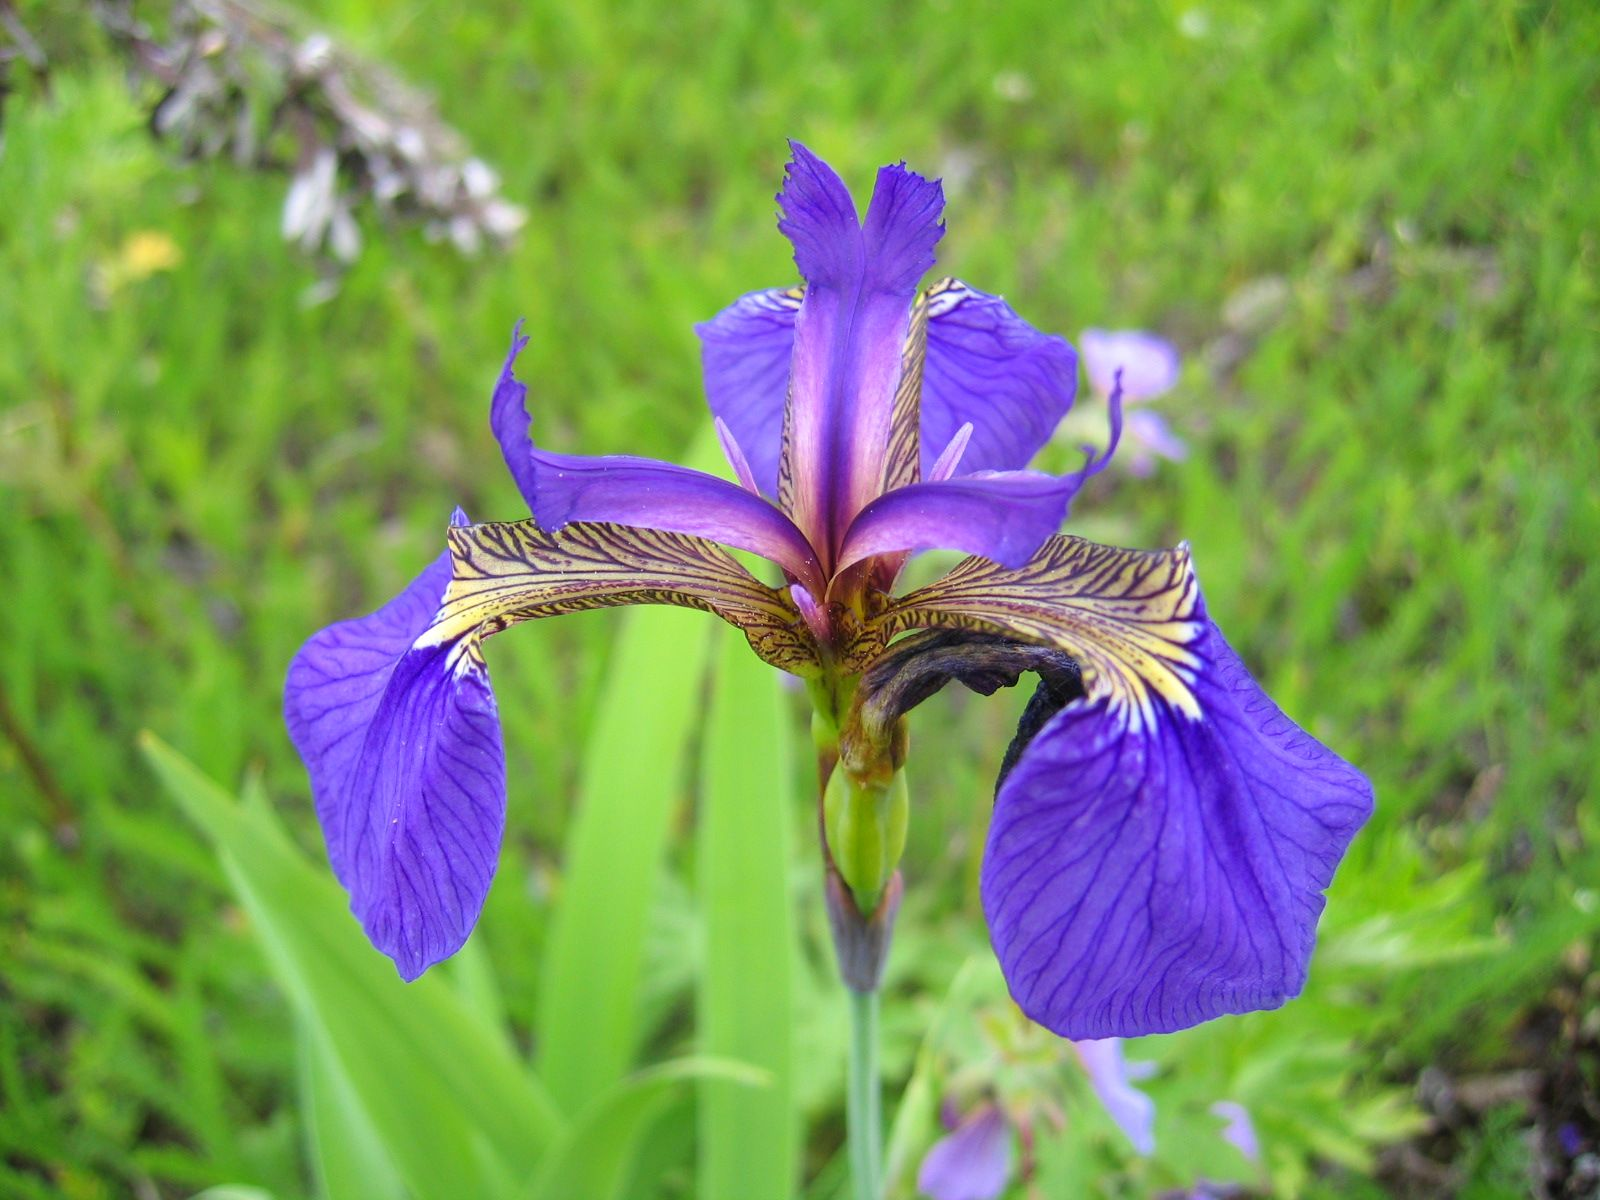
\includegraphics[width=4cm]{setosa}
         \caption{\textit{Iris setosa}}
     \end{subfigure}
     \begin{subfigure}[b]{0.4\textwidth}
         \centering
         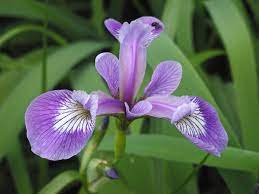
\includegraphics[width=4cm]{versicolor.jpeg}
         \caption{\textit{I.versicolor}}
     \end{subfigure}
        \caption{Two iris species}
        \label{fig:iris}
\end{figure}

\begin{table}[!h]

\caption{\label{tab:iris_data}First few rows in the iris data}
\centering
\begin{tabular}[t]{rrrrl}
\hline
Sepal.Length & Sepal.Width & Petal.Length & Petal.Width & Species\\
\hline
5.1 & 3.5 & 1.4 & 0.2 & setosa\\
4.9 & 3.0 & 1.4 & 0.2 & setosa\\
4.7 & 3.2 & 1.3 & 0.2 & setosa\\
4.6 & 3.1 & 1.5 & 0.2 & setosa\\
5.0 & 3.6 & 1.4 & 0.2 & setosa\\
\hline
\end{tabular}
\end{table}

\hypertarget{fisher-linear-discriminant-analysis}{%
\section{Fisher linear discriminant
analysis}\label{fisher-linear-discriminant-analysis}}

In a 1936 article, \citet{fisher1936} considered the question: what
linear function of the four measurements \begin{equation}
X = \lambda_1 x_1 + \lambda_2 x_2 + \lambda_3 x_3 + \lambda_4 x_4
\end{equation} maximizes the \textit{ratio} of the difference between
the means to the standard deviation within species?

The observed means and their differences are shown in Table
\ref{tab:iris_mean}. We can also compute the sum of squares and products
of deviation from specific means of each species (Table
\ref{tab:compute_var}).

\begin{table}[!h]

\caption{\label{tab:iris_mean}Observed means for two species and their difference (cm.)}
\centering
\begin{tabular}[t]{lrrr}
\hline
Variable & Versicolor & Setosa & Difference\\
\hline
Sepal length & 5.936 & 5.006 & 0.930\\
Sepal width & 2.770 & 3.428 & -0.658\\
Petal length & 4.260 & 1.462 & 2.798\\
Petal Width & 1.326 & 0.246 & 1.080\\
\hline
\end{tabular}
\end{table}

\begin{table}[!h]

\caption{\label{tab:compute_var}Sums of squares and products of four measurements, within species (cm.2)}
\centering
\begin{tabular}[t]{lrrrr}
\hline
  & Sepal length & Sepal width & Petal length & Petal Width\\
\hline
Sepal length & 19.1434 & 9.0356 & 9.7634 & 3.2394\\
Sepal width & 9.0356 & 11.8658 & 4.6232 & 2.4746\\
Petal length & 9.7634 & 4.6232 & 12.2978 & 3.8794\\
Petal Width & 3.2394 & 2.4746 & 3.8794 & 2.4604\\
\hline
\end{tabular}
\end{table}

The linear combination that maximizes \(D^2/S\), where \begin{equation}
D = \lambda_1 d_1 +\lambda_2 d_2+\lambda_3 d_3+\lambda_4 d_4,
\end{equation} where \(d_i\) are the differences between the species
means and \begin{equation}
S = \sum_{p=1}^4\sum_{q=1}^4 \lambda_p\lambda_qS_{pq},
\end{equation} is the solution to a set of linear equations
\begin{equation}
\begin{cases}
S_{11}\lambda_1 + S_{12}\lambda_2 + S_{13}\lambda_3 + S_{14}\lambda_4 = d_1, \\
S_{21}\lambda_1 + S_{22}\lambda_2 + S_{23}\lambda_3 + S_{24}\lambda_4 = d_2, \\ 
S_{31}\lambda_1 + S_{32}\lambda_2 + S_{33}\lambda_3 + S_{34}\lambda_4 = d_3, \\ 
S_{41}\lambda_1 + S_{42}\lambda_2 + S_{43}\lambda_3 + S_{44}\lambda_4 = d_4. \\ 
\end{cases}
\end{equation}

For the iris data, the solution is (-0.03,-0.18,0.22,0.31).

\bibliographystyle{imsart-nameyear}
\bibliography{ims.bib}


\end{document}
